\documentclass[12pt]{article}
\usepackage[utf8]{inputenc}
\usepackage{graphicx} % Allows you to insert figures
\usepackage{amsmath} % Allows you to do equations
\usepackage{fancyhdr} % Formats the header
\usepackage{geometry} % Formats the paper size, orientation, and margins
\usepackage{color} % color of fonts
\usepackage[colorlinks,linkcolor=blue]{hyperref} % for hyperlink
\usepackage{caption} % for subfigure
\usepackage{subfigure} % for subfigure
\linespread{1.25} % about 1.5 spacing in Word
\setlength{\parindent}{0pt} % no paragraph indents
\setlength{\parskip}{1em} % paragraphs separated by one line
\usepackage[style=authoryear-ibid,backend=biber,maxbibnames=99,maxcitenames=2,uniquelist=false,isbn=false,url=true,eprint=false,doi=true,giveninits=true,uniquename=init]{biblatex} % Allows you to do citations - does Harvard style and compatible with Zotero
\usepackage{algorithm} % for pseudo code
\usepackage{algpseudocode} % for pseudo code
\usepackage{wrapfig}
\urlstyle{same} % makes a nicer URL and DOI font 
\AtEveryBibitem{
    \clearfield{urlyear}
    \clearfield{urlmonth}
} % removes access date
\AtEveryBibitem{\clearfield{month}} % removes months in bibliography
\AtEveryCitekey{\clearfield{month}} % removes months in citations
\renewbibmacro{in:}{} % Removes the "In" before journal names

\renewbibmacro*{editorstrg}{%from biblatex.def
  \printtext[editortype]{%
    \iffieldundef{editortype}
      {\ifboolexpr{
         test {\ifnumgreater{\value{editor}}{1}}
         or
         test {\ifandothers{editor}}
       }
         {\bibcpstring{editors}}
         {\bibcpstring{editor}}}
      {\ifbibxstring{\thefield{editortype}}
         {\ifboolexpr{
            test {\ifnumgreater{\value{editor}}{1}}
            or
            test {\ifandothers{editor}}
          }
            {\bibcpstring{\thefield{editortype}s}}%changed
            {\bibcpstring{\thefield{editortype}}}}%changed
         {\thefield{editortype}}}}}

\renewbibmacro*{byeditor+others}{%from biblatex.def
  \ifnameundef{editor}
    {}
    {\printnames[byeditor]{editor}%
     \addspace%added
     \mkbibparens{\usebibmacro{editorstrg}}%added
     \clearname{editor}%
     \newunit}%
  \usebibmacro{byeditorx}%
  \usebibmacro{bytranslator+others}}
  % The commands above from lines 20-49 change the way editors are displayed in books
\AtEveryBibitem{%
  \clearlist{language}%
} % removes language from bibliography
\citetrackerfalse 
% Removes ibids (ibidems)
\DeclareNameAlias{sortname}{family-given} % Ensures the names of the authors after the first author are in the correct order in the bibliography
\renewcommand*{\revsdnamepunct}{} % Corrects punctuation for authors with just a first initial
\addbibresource{Example.bib} % Tells LaTeX where the citations are coming from. This is imported from Zotero
\usepackage[format=plain,
            font=it]{caption} % Italicizes figure captions
\usepackage[english]{babel}
\usepackage{csquotes}
\renewcommand*{\nameyeardelim}{\addcomma\space} % Adds comma in in-text citations
\renewcommand{\headrulewidth}{0pt}
\geometry{letterpaper, portrait, margin=1in}
\setlength{\headheight}{14.49998pt}

\newcommand\titleofdoc{3D modelling Assignment 2} %%%%% Put your document title in this argument
\newcommand\GroupName{GEO1004} %%%%% Put your group name here. If you are the only member of the group, just put your name

\begin{document}
\begin{titlepage}
   \begin{center}
        \vspace*{4cm} % Adjust spacings to ensure the title page is generally filled with text

        \Huge{\titleofdoc} 

        \vspace{0.5cm}
        \LARGE{Enriching the 3D BAG with new attributes}
            
        \vspace{3 cm}
        \Large{GEO1004}
       
        \vspace{0.25cm}
        \large{
        Yitong Xia 5445825
        \\Yue Yang 5516862
        \\Fengyan Zhang 5462150}
       
        \vspace{3 cm}
        \Large{03 20, 2022}
        
        \vspace{0.25 cm}
        \Large{GEO1004}
       

       \vfill
    \end{center}
\end{titlepage}

\setcounter{page}{2}
\pagestyle{fancy}
\fancyhf{}
\rhead{\thepage}
\lhead{\GroupName; \titleofdoc}

\section{Methodology} % If you want numbered sections, remove the star after \section

On the whole, we use \href{https://github.com/cityjson/cjio/tree/develop}{cjio (develop branch)} as an auxiliary tool to clean up and triangulate files. And we mainly use two inputs and outputs to calculate volume, floor, area and orientation respectively. The main process is as follows.

\begin{figure}[ht] % h - Place the float here, i.e., approximately at the same point it occurs in the source text (however, not exactly at the spot)
\centering
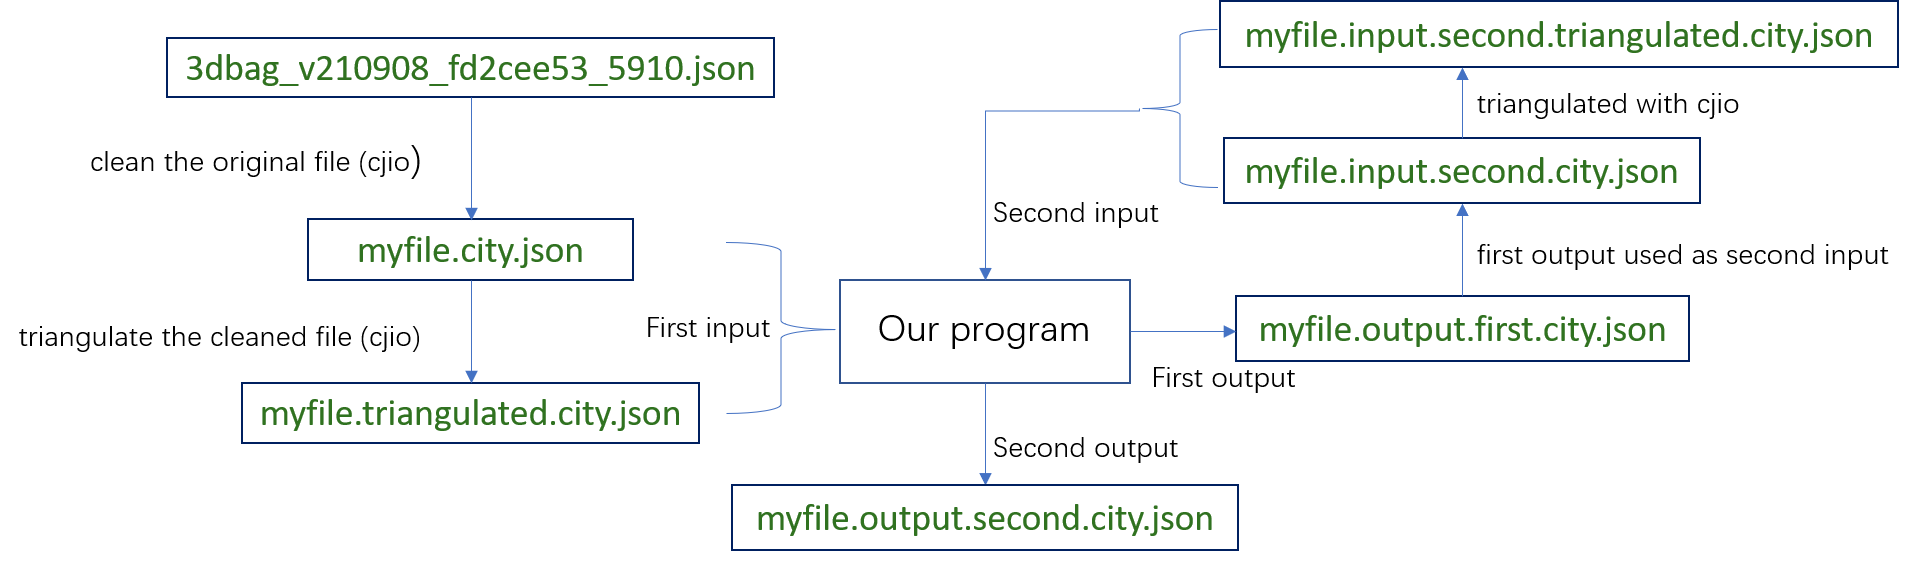
\includegraphics[width=16cm]{methodology-1.png}
\caption{Overview Methodology}
\end{figure}

The reason why we have two inputs is that we use triangles to calculate the area of each roof surface and select the corresponding normal vector to estimate the orientations (which will be described in the corresponding chapters later). This requires us to identify which triangles (in the triangulated file) belong to which roof surface in the original file, therefore two inputs are needed.

In the first input, we use \textcolor{black}{\textit{myfile.city.json}} file to calculate the floor and its corresponding triangulated file (\textcolor{black}{\textit{myfile.triangulated.city.json}}) to calculate the volume. At the same time, we establish a unique \href{https://www.cityjson.org/specs/1.1.1/#semantics-of-geometric-primitives}{Semantic Object} for each face belonging to \textit{RoofSurface}. We then write the calculation results and the new semantic objects into the first output file.

In the input of the second step, we use the file \textcolor{black}{\textit{myfile.input.second.city.json}} and its corresponding triangulated file \textcolor{black}{\textit{myfile.input.second.triangulated.city.json}} to calculate the area and orientation, and write the calculation results into the output file of the second input.

After having the result file in the second output, \href{https://validator.cityjson.org/}{cjval} and \href{http://geovalidation.bk.tudelft.nl/val3dity/}{val3dity} are used for verification. We need to process the invalid buildings according to the error report (can be downloaded from \href{http://geovalidation.bk.tudelft.nl/val3dity/}{val3dity}). The relevant process is as follows(see Fig. 2).

\begin{figure}[ht] % h - Place the float here, i.e., approximately at the same point it occurs in the source text (however, not exactly at the spot)
\centering
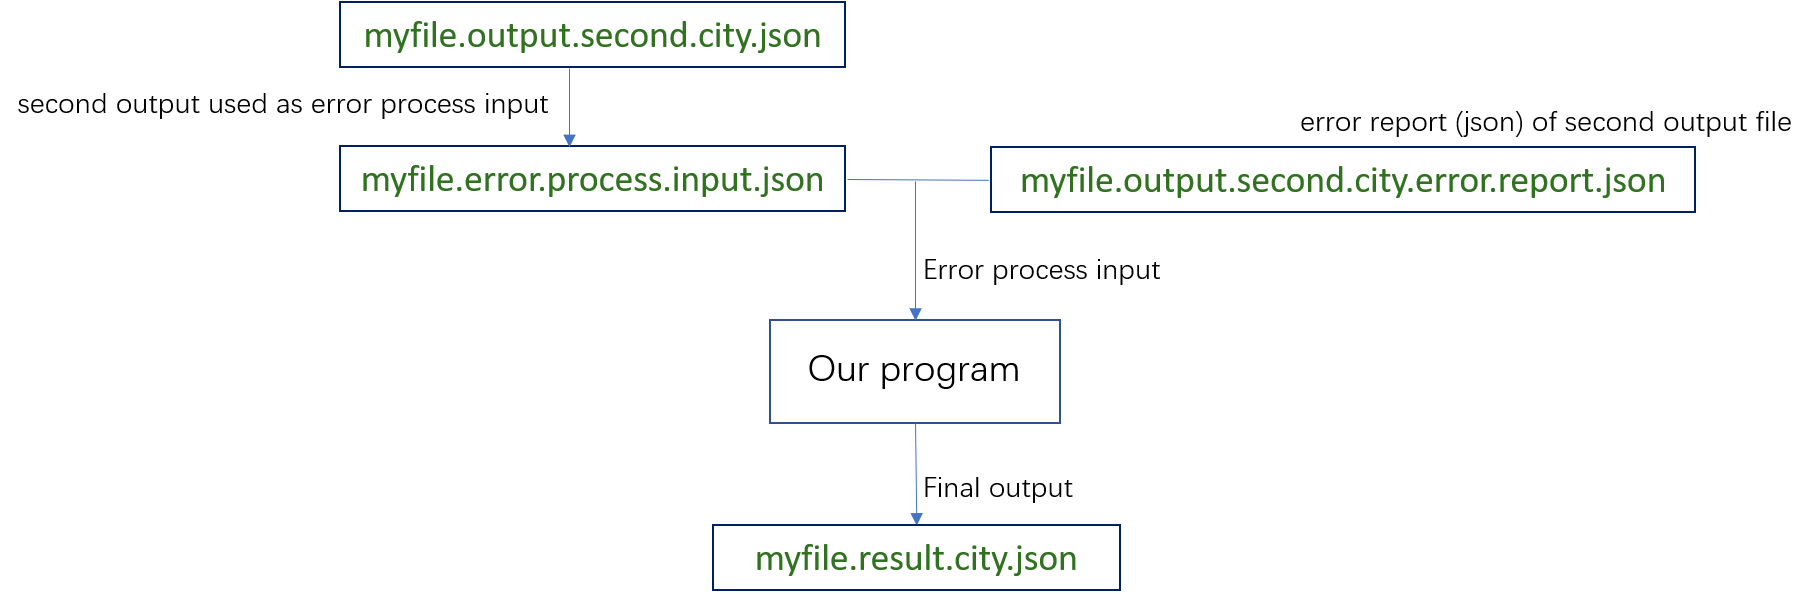
\includegraphics[width=16cm]{methodology-error process.png}
\caption{Error Process}
\end{figure}

After error processing, the final outcome file (\textcolor{black}{\textit{myfile.result.city.json}}) can be obtained. More descriptions are in the corresponding chapter.

\section{Volume}
Because the shape of buildings is mostly irregular, the initial idea is to decompose each building into tetrahedrons, and then calculate the volume of each tetrahedron to obtain the volume of the whole building. However, in practice, we found that for buildings with arbitrary shape and irregularity, it is difficult to select a random point outside and then form tetrahedrons with the vertices of the building. The artificially specified external point forms a tetrahedron with every three points in the vertex sequence of each building, but this is not universal, different building structures will affect the order of vertices when constructing tetrahedrons(see Fig. 3).
\begin{figure}[ht] % h - Place the float here, i.e., approximately at the same point it occurs in the source text (however, not exactly at the spot)
\centering
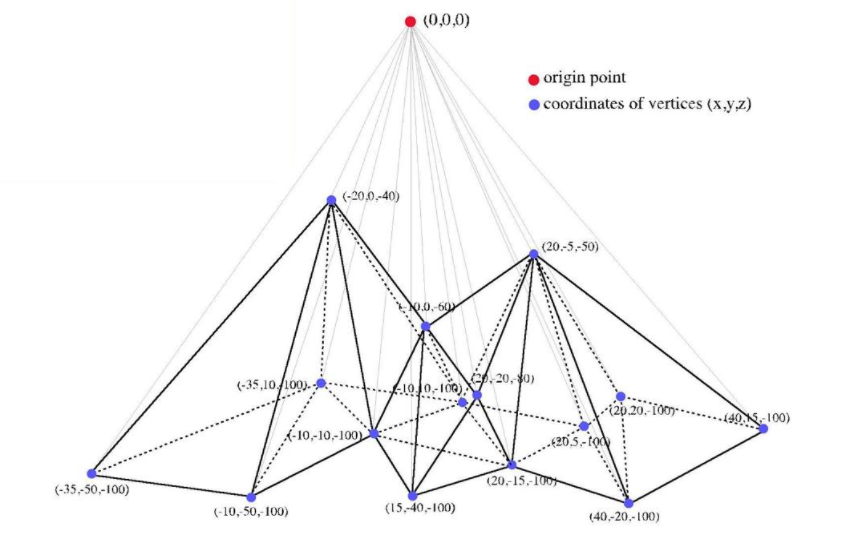
\includegraphics[width=10cm]{decompose_to_tetrahedra.png}
\caption{Construct Tetrahedrons(From \href{https://ysjournal.com/tetrahedral-shoelace-method-calculating-volume-of-irregular-solids/}{Tetrahedral Shoelace Method})}
\end{figure}
Later, we found that in the actual calculation, manually dividing the building into tetrahedrons is not necessary. When the vertex order of all faces is the same when observed from a reference point (all clockwise or counterclockwise), then the volume can be calculated by using the following formula when traversing each triangulated face:
\begin{equation} % add * after equation for unnumbered equations
     V = \frac{1}{6}\times \left | det\begin{bmatrix}
    v1\\ 
    v2\\ 

    v3\end{bmatrix} \right |
\end{equation}
The algorithm goes as follows:
\begin{algorithm}
\caption{algorithm for volume}
\begin{algorithmic}
\For{each Building Part} 
    \State $V \gets 0$
    \For{each triangle IN each Surface}
        \State $v1 \gets triangle[0]$ \Comment{$v1$, $v2$, $v3$ indicates the three vertices of the triangle}
        \State $v2 \gets triangle[1]$
        \State $v3 \gets triangle[2]$
        \State $V \mathrel{+}= (1/6)\times \left | det\begin{bmatrix}
        v1 &  v2& v3
        \end{bmatrix}^ \mathrm{ T }  \right |$
    \EndFor
\EndFor
\end{algorithmic}
\end{algorithm}

For invalid \textit{BuildingPart}, volume is set to \textit{null}.

\section{Floor}
When calculating the floor, we only calculated those CityObjects whose type is \textit{Building}. To calculate the height of the roof, we read ``h\_dak\_max'' and ``h\_dak\_min'' and ``h\_maaiveld'' of each building from the attributes and apply the formula below:
\begin{equation} % add * after equation for unnumbered equations
     Floor = \frac{((``h\_dak\_max" - ``h\_dak\_min")\times 0.7)+(``h\_dak\_min" - ``h\_maaiveld")}{3.0}
\end{equation}
where 3.0 is the typical height of ceilings, we need to round the value to the nearest integer after the calculation.

We think the step of converting the result of the calculation to an integer is worth noting; if we convert the data type with int(), we will not get the correct result because it simply removes the decimal part. If the decimal part is greater than 0.5, we round the value to the next integer; if the decimal part is less than 0.5, we round the value to the current integer.

In the result file, the value of floor is set to $null$ in three buildings without geometry.

\section{Area}
For calculating the area of the roof surfaces, surface triangulation method is selected to complete the area calculation, as it is easier and more accurate to calculate the area of a triangle (using Heron's formula) than that of a polygon. At the same time, triangulation can well solve the problem of holes inside the surfaces. We tested the cjio triangulation using a roof surface with a hole and proved that triangulation can avoid the holes well in the triangulation process(see Fig. 4).

\begin{figure}[h] % h - Place the float here, i.e., approximately at the same point it occurs in the source text (however, not exactly at the spot)
\centering
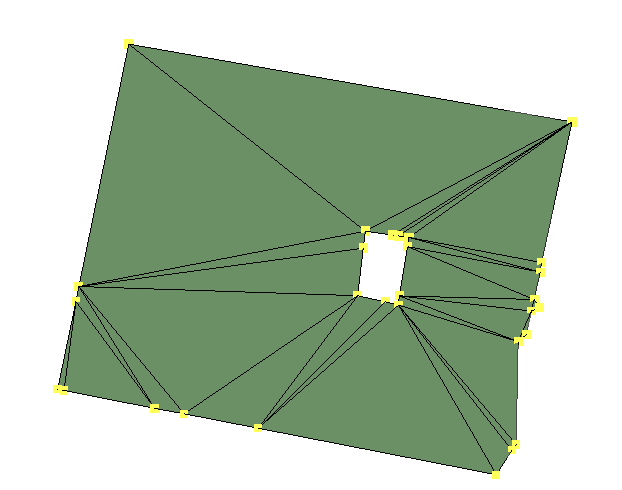
\includegraphics[width=10cm]{roofArea.png}
\caption{The Triangulation of the Roof Surface Can Prevent the ``Hole" Well}
\end{figure}

Before calculating the area, creating new and unique semantic objects for surfaces which belong to \textit{RoofSurface} is needed. In this way, each roof surface has a corresponding semantic object. At the same time, updating the index value of the corresponding new semantic surface in the \textit{value} array.
After all the new semantic surfaces are created, export the current json file and triangulate it using cjio. The following command for triangulation is used:

\texttt{cjio myfile.city.json triangulate save myfile.triangulated.city.json}

Then two files can be built, one is \textcolor{black}{\textit{myfile.output.first.city.json
}}, another one is the corresponding triangulated json file. Now we start iterating each \textit{geometry} whose type is \textit{Solid} in the triangulated json file, calculate the area of each triangle whose type is \textit{RoofSurface}, and accumulate the areas to the corresponding roof surface. After finishing calculating the area of all triangles in one geometry, we assign the summed values to the corresponding \textit{RoofSurface} in the \textcolor{black}{\textit{myfile.output.first.city.json}} file. 

Overall, we have completed the area calculation with the aid of the triangulation.

Another method has been tested as well, a brief explanation is to first calculate the projected area of each roofsurface in the XY plane (pay attention to subtracting the inner ring area), and then convert the plane area into the area of this face according to the angle between this face and the XY plane.

\subsubsection*{Results Analysis}
To validate our results, the area of surfaces in the file \textcolor{black}{\textit{myfile.city.json}} is checked through \href{https://www.meshlab.net/}{MeshLab}. It is found that our results are close to area computations in the software, but there are still some differences. Taking NL.IMBAG.Pand.0503100000004247 that contains three roof surfaces as an example, for each surface, our results are 44.53, 2.33, 42.63, while the result given by \href{https://www.meshlab.net/}{MeshLab} are around 44.48,  2.38, 42.70 respectively. It may be because the operation of geometric calculation, depending on the algorithm, inevitably leads to different degrees of loss. In addition, we reconstruct the roof surfaces using an obj file generated with the coordinates output from the code and check it in the software, in comparison with  the obj file exported from \textcolor{black}{\textit{myfile.city.json}} using cjio. We find the latter surfaces are smoother, which may also prove the loss of numerical accuracy in the calculation. 


\begin{figure}[htbp]
\centering
\subfigure[The File Generated from the Code]
{
	\begin{minipage}{7cm}
	\centering     
	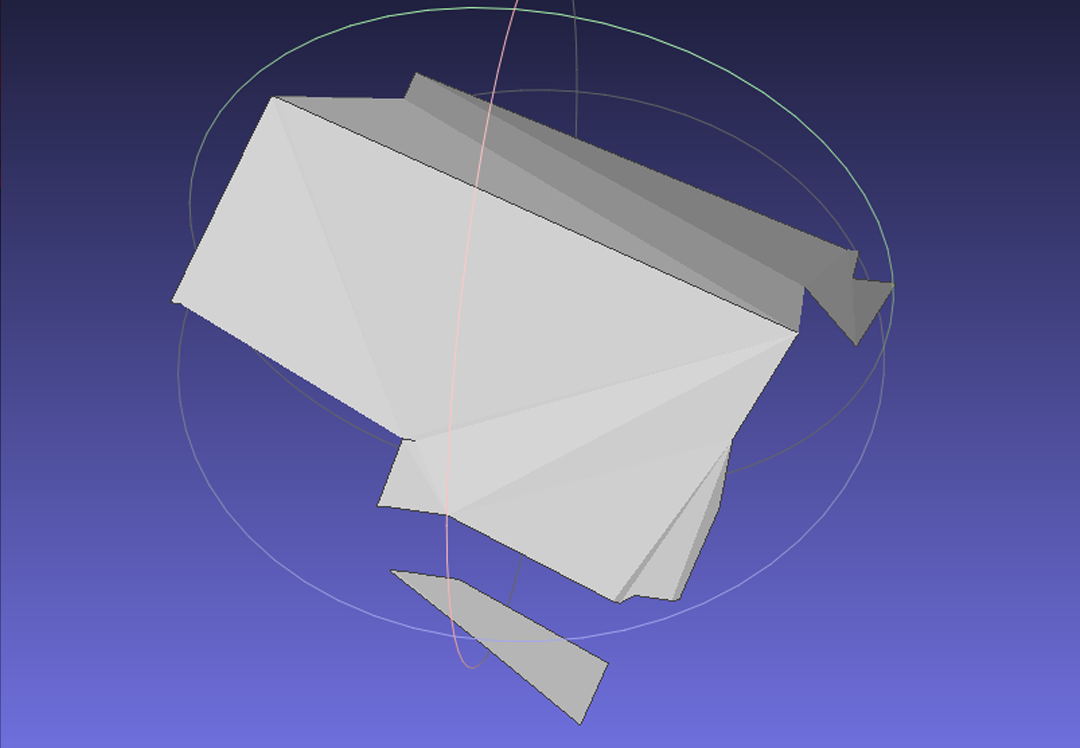
\includegraphics[height=5cm,width=6cm]{figure/roofreconstruct.PNG}
	\end{minipage}
}
\subfigure[The File Exported from cjio]
{
	\begin{minipage}{7cm}
	\centering
	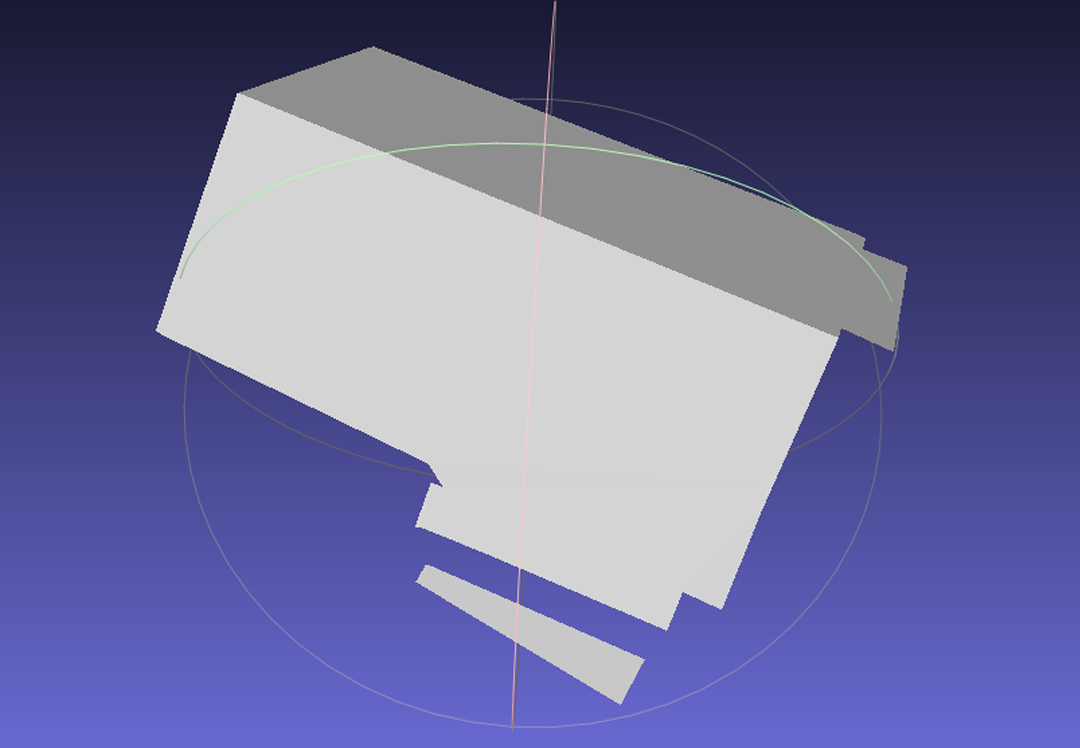
\includegraphics[height=5cm,width=6cm]{figure/rooffromcjio.PNG}
	\end{minipage}
}
\caption{Comparison of Surfaces}
\end{figure}

\section{Orientation}

Each \textit{RoofSurface} will have its own normal vector. By projecting this normal vector onto the XY plane, a 2D vector or a point (when the \textit{RoofSurface} is horizontal) can be obtained. The positive direction of the y-axis is set to the north direction, and the direction of the 2D vector can be determined by the sign of the XY coordinate and the included angle between the 2D vector and the y-axis (see eq. (3) and Algorithm. 2).
\begin{equation} % add * after equation for unnumbered equations
     \alpha = \arctan \left ( x/  y \right )
\end{equation}
Before applying this formula, it is necessary to judge whether the \textit{RoofSurface} is horizontal or not by comparing the length of the normal vector projected onto the XY plane with a manually set threshold. Please note that the value of this threshold can be changed, after randomly selecting buildings for testing, we set the threshold to 1. The process of estimating orientations is as follows.
\begin{algorithm}[ht]
\begin{algorithmic}
\caption{algorithm for orientation}
\If {$length< horizontal\_epsilon$}
    \State $orientation\gets ``horizontal"$
\Else
    \If {$\left | y \right |= 0$}
        \If {$x > 0$}
            \State $orientation\gets ``EN"$
        \Else
            \If{$\left | x \right |= 0$}
                \State $orientation\gets ``horizontal"$
            \Else
                \State $orientation\gets ``WN"$
            \EndIf
        \EndIf
    \Else \Comment{$y\neq 0$}
        \State $quadrant\gets 1,2,3,4$ \Comment{four quadrants assigned by the sign of xy coordinates}
        \State $\alpha = \arctan \left ( x/  y \right )$
        \State $orientation\gets result$ \Comment{use $\alpha$ and quadrant to decide the orientation value}
    \EndIf
\EndIf
\end{algorithmic}
\end{algorithm}
The direction of the \textit{RoofSurface} to which the normal vector belongs can be determined by the quadrant where the normal vector is projected and the included angle with the y-axis (which can be positive or negative, see Fig. 6).
\begin{figure}[ht] % h - Place the float here, i.e., approximately at the same point it occurs in the source text (however, not exactly at the spot)
\centering
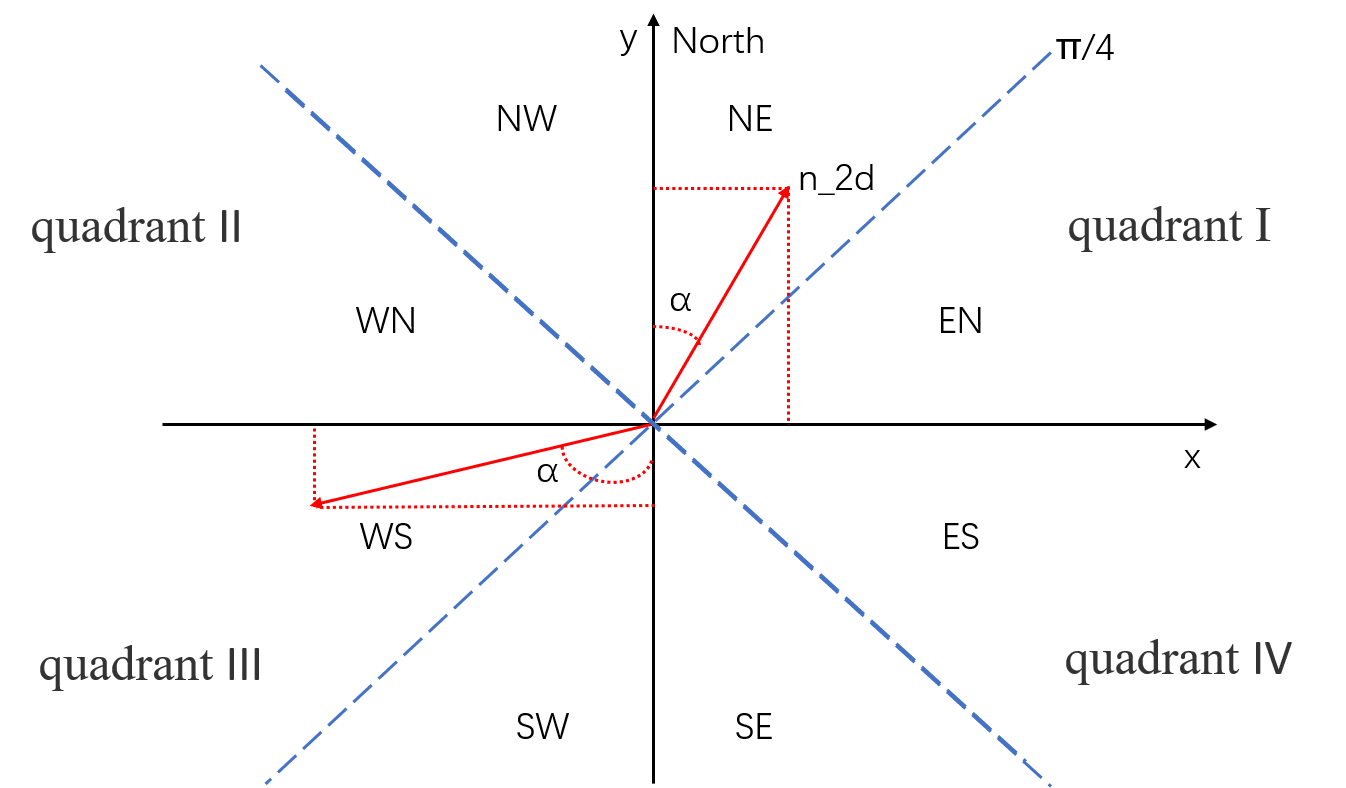
\includegraphics[width=10cm]{figure/orientation-method.png}
\caption{Orientation}
\end{figure}

When calculating the normal vector, we need to ensure that the direction of the normal vector is correct, so the triangulated file of the second input is used. At the same time, due to the existence of conservative points, for each triangle constituting each face, three vertices may be collinear (for instance, two of the three vertices are repeated). In order to ensure that the normal vector can be calculated correctly, the three vertices of the triangle with the largest area are selected(see Fig. 7).
\begin{figure}[htbp]
\centering
\subfigure[Max Triangle-1]
{
	\begin{minipage}{7cm}
	\centering
	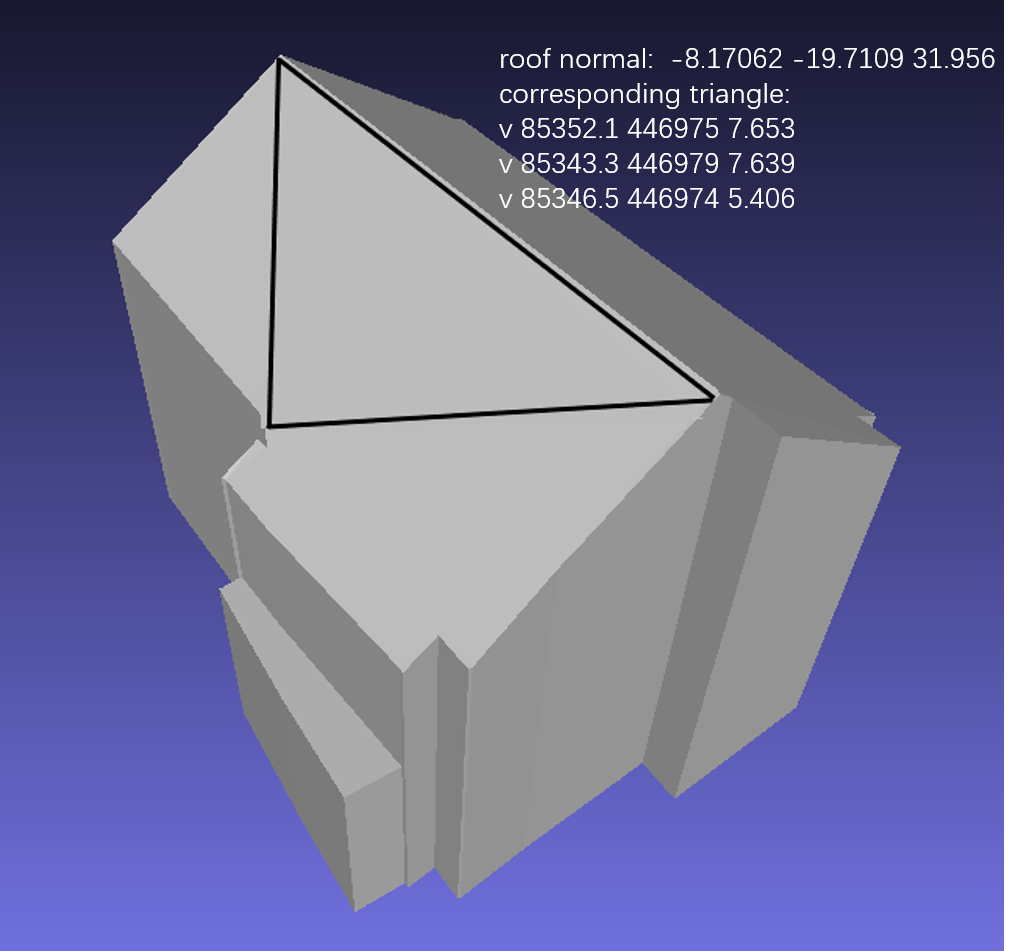
\includegraphics[height=6cm,width=7cm]{figure/maxtriangle-1.png}
	\end{minipage}
}
\subfigure[Max Triangle-2]
{
	\begin{minipage}{7cm}
	\centering     
	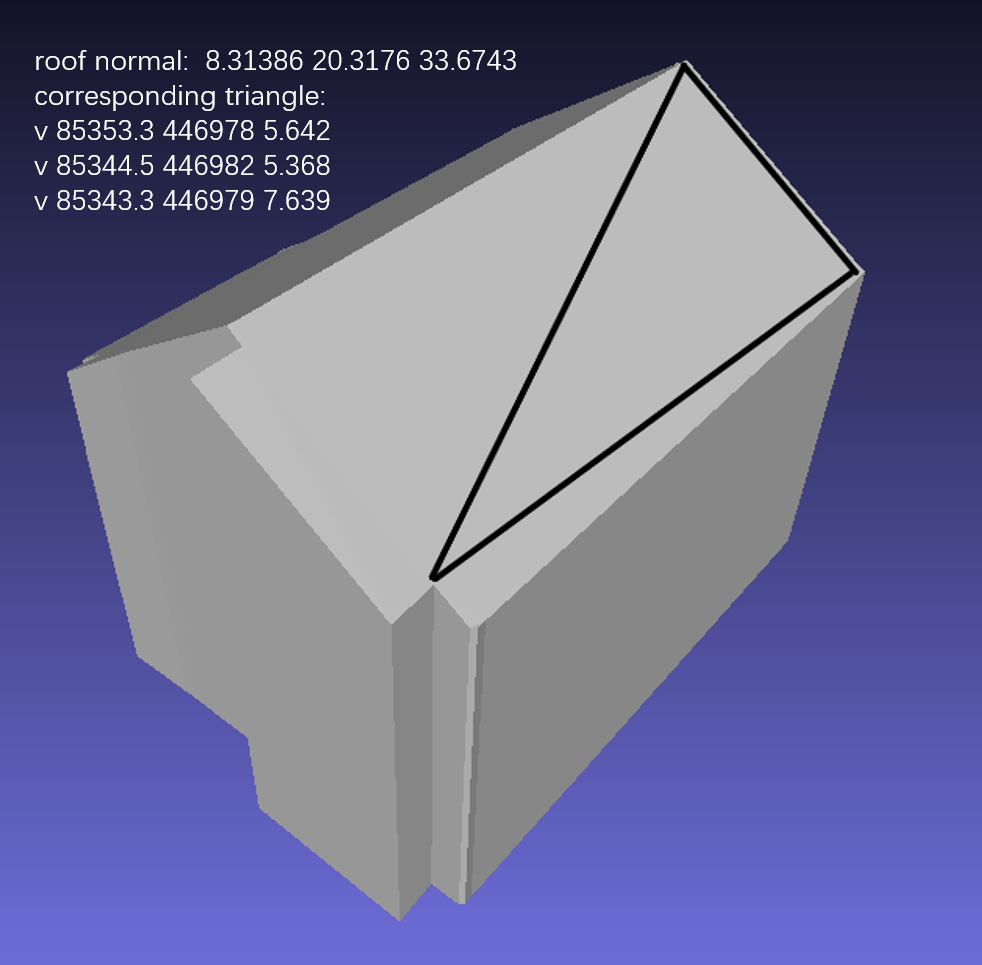
\includegraphics[height=6cm,width=7cm]{figure/maxtriangle-2.png}
	\end{minipage}
}
\caption{Vertices of Max Triangles}
\end{figure}
\section{Invalid Cases}
\subsubsection*{Invalid Geometry}

In the input file \textcolor{black}{\textit{myfile.city.json}}, we use \href{http://geovalidation.bk.tudelft.nl/val3dity/}{val3dity} to check its geometry and find that there are some invalid buildings, as shown below(see Fig. 8). We try to export the specific invalid building as an \href{https://docs.fileformat.com/3d/obj/}{OBJ} file and then open it in \href{https://www.meshlab.net/}{MeshLab} to observe the invalid part. The main categories and examples are as follows.

\begin{figure}[h] % h - Place the float here, i.e., approximately at the same point it occurs in the source text (however, not exactly at the spot)
\centering
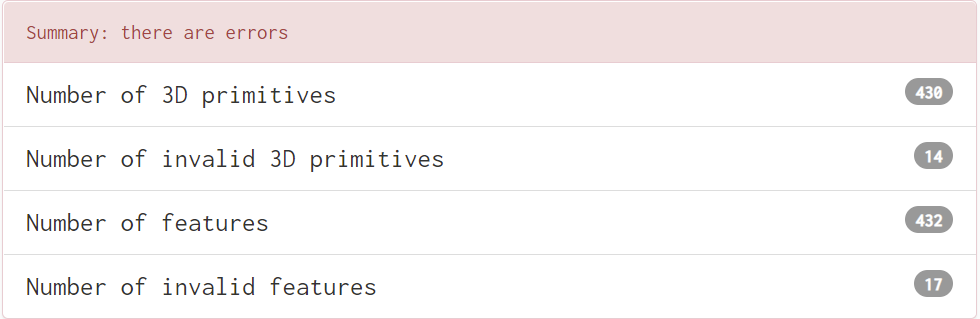
\includegraphics[width=10cm]{val3dityerror.PNG}
\caption{Error Summary in \textcolor{black}{\textit{myfile.city.json}}}
\end{figure}
$Consecutive Points Same$(\href{https://val3dity.readthedocs.io/en/latest/errors/#consecutive-points-same}{details})

In short, there are consecutive vertices with very similar positions, or two repeated vertices with the same coordinates in the file(see Fig. 9(a)).
\begin{figure}[htbp]
\centering
\subfigure[Consecutive Points Example]
{
	\begin{minipage}{7cm}
	\centering
	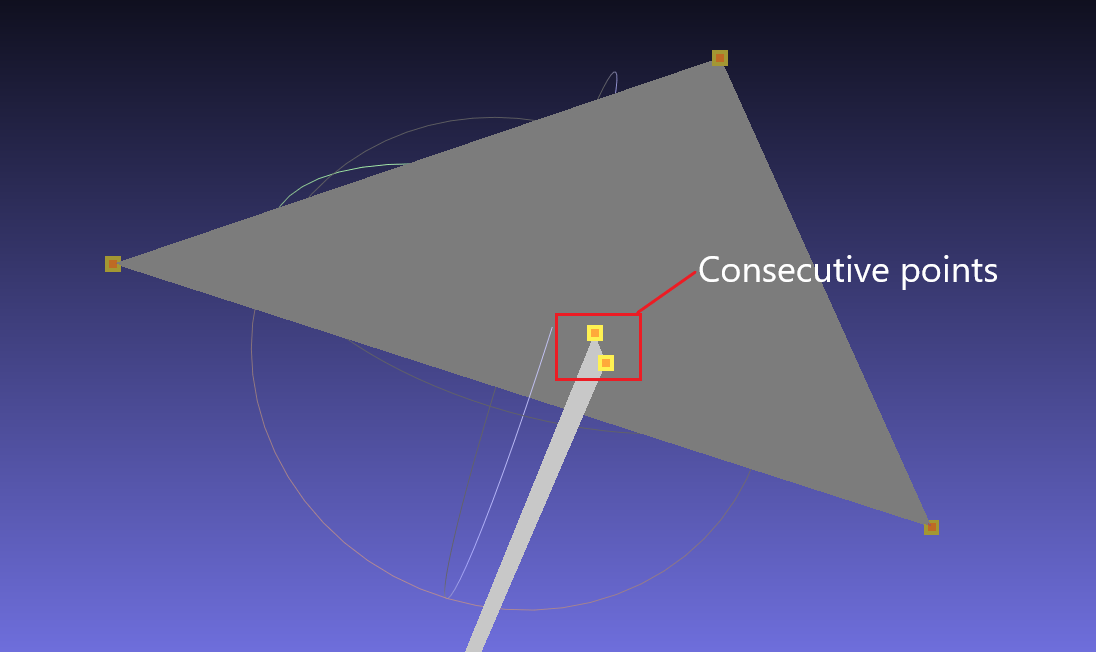
\includegraphics[height=6cm,width=7cm]{error102.NL.IMBAG.Pand.0503100000018414(0).png}
	\end{minipage}
}
\subfigure[Ring Self Intersection Example]
{
	\begin{minipage}{7cm}
	\centering     
	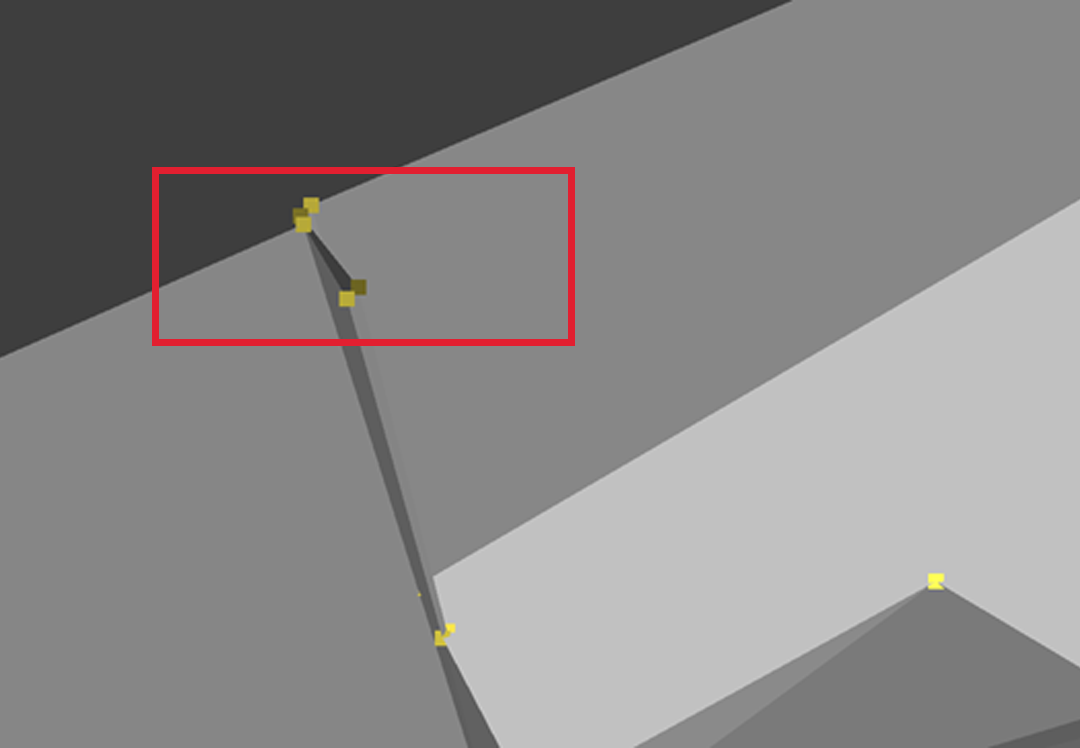
\includegraphics[height=6cm,width=7cm]{figure/Ring Self Intersection.png}
	\end{minipage}
}
\caption{Examples}
\end{figure}

$Ring Self Intersection$(\href{https://val3dity.readthedocs.io/en/latest/errors/#ring-self-intersection}{details})

There are self intersecting rings or, for instance, rings that are (partially) collapsed to a line in the file (see Fig. 9(b)).

$Non Planar Polygon Normals Deviation$(\href{https://val3dity.readthedocs.io/en/latest/errors/#non-planar-polygon-normals-deviation}{details})

The deviation normals of the following two files exceeds the limit tolerance (see Fig. 10)
\begin{figure}[htbp]
\centering
\subfigure[Example-1]
{
	\begin{minipage}{7cm}
	\centering
	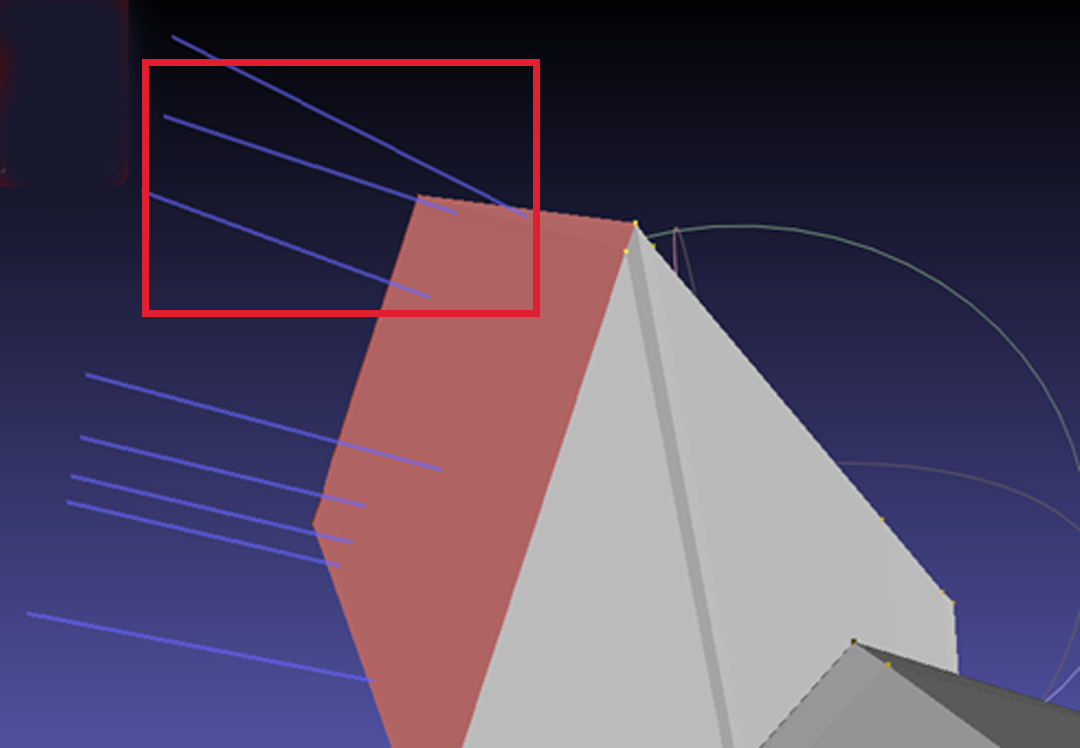
\includegraphics[height=5cm,width=6cm]{figure/Non Planar Polygon Normals Deviation01.PNG}
	\end{minipage}
}
\subfigure[Example-2]
{
	\begin{minipage}{7cm}
	\centering     
	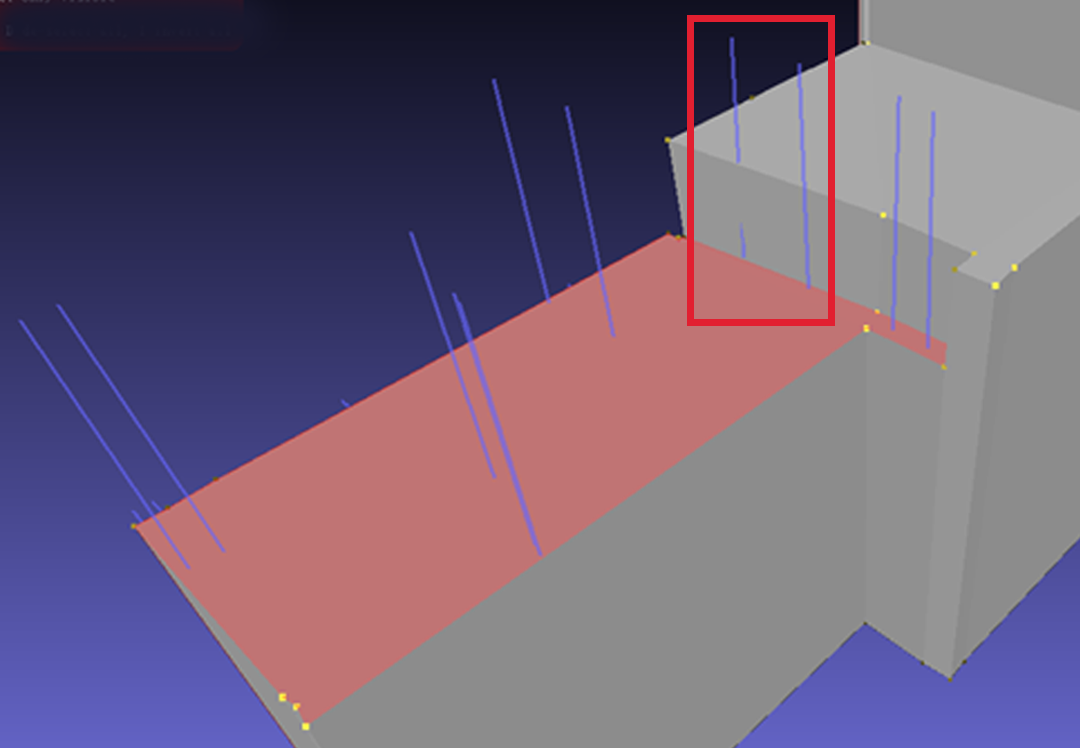
\includegraphics[height=5cm,width=6cm]{figure/Non Planar Polygon Normals Deviation02.PNG}
	\end{minipage}
}
\caption{Non Planar Polygon Normals Deviation}
\end{figure}

$Shell Not Closed$(\href{https://val3dity.readthedocs.io/en/latest/errors/#shell-not-closed}{details})

The shell in the building part contains ``holes"(see Fig. 11).
\begin{figure}[htbp]
\centering
\subfigure[NL.IMBAG.Pand.0503100000020272]
{
	\begin{minipage}{7cm}
	\centering
	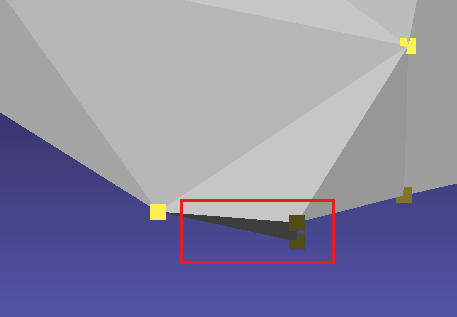
\includegraphics[height=5cm,width=6cm]{figure/error302.NL.IMBAG.Pand.0503100000020272.MeshLab.PNG}
	\end{minipage}
}
\subfigure[NL.IMBAG.Pand.0503100000020272]
{
	\begin{minipage}{7cm}
	\centering     
	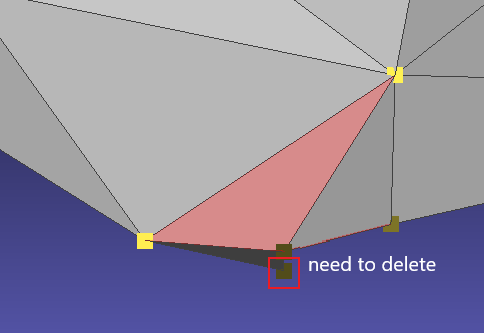
\includegraphics[height=5cm,width=6cm]{figure/error302.NL.IMBAG.Pand.0503100000020272.MeshLab.connected.PNG}
	\end{minipage}
}
\caption{Shell Not Closed}
\end{figure}
% figure

$Non Manifold Case$(\href{https://val3dity.readthedocs.io/en/latest/errors/#non-manifold-case}{details})

This error might be returned for shells having an edge shared by more than two faces, also in cases where surfaces of shells are inconsistently oriented (see Fig. 12).

\begin{figure}[htbp]
\centering
\subfigure[nonmanifold.31387-1]
{
	\begin{minipage}{7cm}
	\centering
	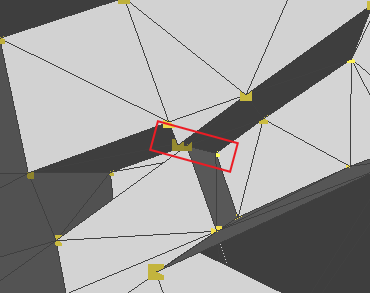
\includegraphics[height=5cm,width=6cm]{figure/nonmanifold.31387-2.png}
	\end{minipage}
}
\subfigure[nonmanifold.31387-1]
{
	\begin{minipage}{7cm}
	\centering     
	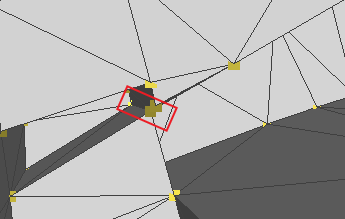
\includegraphics[height=5cm,width=6cm]{figure/nonmanifold.31387-3.png}
	\end{minipage}
}
\caption{Non Manifold Case}
\end{figure}
\subsubsection*{Invalid Building Impact}
We also check the geometry in the file \textcolor{black}{\textit{myfile.triangulated.city.json}} using \href{http://geovalidation.bk.tudelft.nl/val3dity/}{val3dity}. It is found that there are still some invalid buildings, as shown below(see Fig. 13). After triangulation, the two buildings which were reported as the error ``NON PLANAR POLYGON NORMALS DEVIATION" are considered valid, the building that introduced ``RING SELF INTERSECTION" is still considered invalid and returns the error ``NON MANIFOLD CASE", which might also account for the reason why the area of the roof surface (``roof id": ``NL.IMBAG.Pand.0503100000033695-0.roof.2") is null.
\begin{figure}[htbp] 
\centering
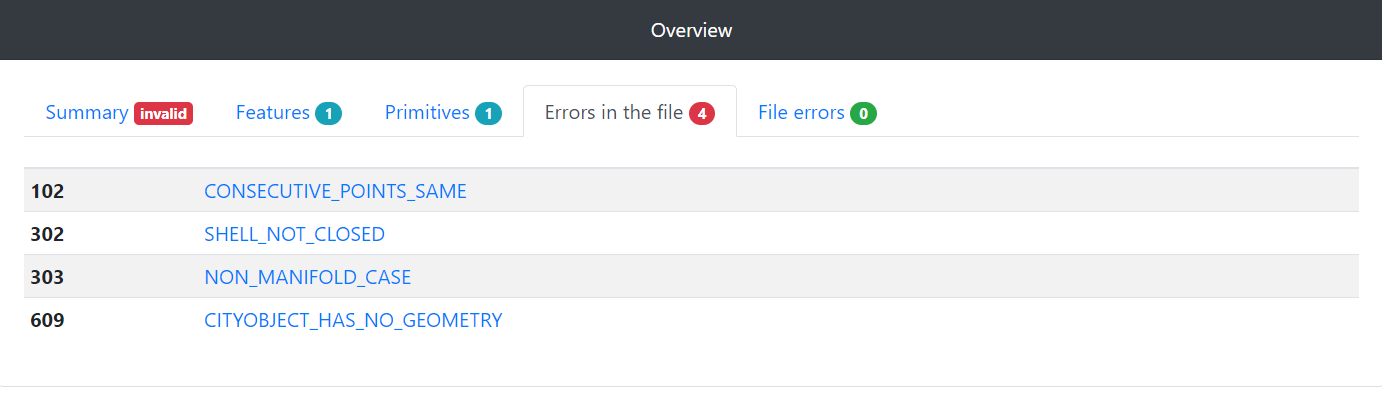
\includegraphics[width=10cm]{overview of the validation report.PNG}
\caption{Overview of Validation in \textcolor{black}{\textit{myfile.triangulated.city.json}}}
\end{figure}

The impact of the six errors not eliminated in the original document on the four attributes is evaluated as follows

\begin{center}
\begin{tabular}{ |c|c|c|c|c| } 
 \hline
 error type & Volume & Floor & Area & Orientation \\ 
 \hline
 Consecutive Points Same & - & - & - & + \\ 
 \hline
 Ring Self Intersection & + & - & + & + \\ 
 \hline
 Non Planar Polygon Normals Deviation & - & - & - & + \\ 
 \hline
 Shell Not Closed & + & - & - & - \\ 
 \hline
 Non Manifold Case & - & - & - & - \\ 
 \hline
 CityObject Has No Geometry & + & + & + & + \\ 
 \hline
\end{tabular}
\end{center}

The $+$ sign represents a great influence (which may lead to failure of calculation or great difference in calculation accuracy), and the $-$ sign represents a small influence.

The specific impact needs further analysis in the future.
\section{Workload}

Yitong did the floor calculation, Yue Yang did the area calculation, Fengyan did the volume and orientation calculation.

For area calculation, we tried multiple methods and worked on the area part together.

We write the report together.

\section{Appendix}

The relevant code is in this
\href{https://github.com/SEUZFY/CityJSON}{git repository}.

In our result file, $floor$ and $volume$ are written in Building $->$ attributes. In semantics $->$ surfaces, each $RoofSurface$ contains two area attributes:

$area$ : area calculated using projection method.

$area\_tri$ : area calculated using triangulation method.

Both area values are kept because we want to compare and analyze the accuracy of the two different methods. 
\end{document}
